\section[Ход работы]{ХОД РАБОТЫ}

\subsection{Описание предметной области}

В качестве предметной области данной расчетной работы выберем
описание и автоматизацию учета данных бизнес-процессов организации,
ведущей учет своих сотрудников.

Объектом предметной области можно считать \texttt{Сотрудника}, занимающего
одну или несколько \texttt{Должностей}.


\subsection{Создание перечислений}

Сущность <<Сотрудник>> имеет определенный уровень образования, множество значений
которого удобно показать используя перечисление <<Образования>>, изображенного
на рисунке~\ref{fig:enum}.
\begin{figure}[h!]
  \centering
  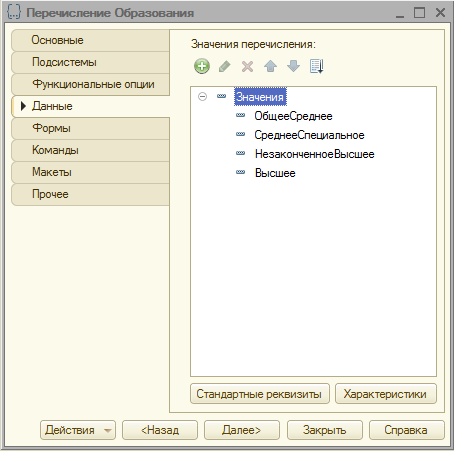
\includegraphics[width=120mm]{pic/enum}
  \caption{Значения перечисления <<Образования>>}
  \label{fig:enum}
\end{figure}

Создание перечислений производится с помощью раздела <<Перечисления>>
панели <<Конфигурация>> режима <<Конфигуратор>>. Для создания
перечисления необходимо, щелкнув правой кнопкой мыши по этому
разделу, выбрать пункт <<Добавить>>. Далее в появившемся окне
следует определить имя и синоним перечисления.
После этого в разделе <<Данные>> необходимо определить возможные
значения создаваемего перечисления.

Созданные перечисления призваны сэкономить время и снизить количество
ошибок при заполнении справочников.

\subsection{Создание справочников}

Создание справочников производится с помощью раздела <<Справочники>>
панели <<Конфигурация>> режима <<Конфигуратор>>.
Для создания справочника необходимо, щелкнув правой кнопкой мыши по этому
разделу, выбрать пункт <<Добавить>>. Далее в появившемся окне
следует определить имя и синоним справочника.
После этого в разделе <<Данные>> необходимо определить структуру
хранимых данных путем добавления и указания свойств реквизитов
и табличных частей.

В разрабатываемой информационной системе справочники соответствуют
объектам предметной области: <<Сотрудники>>, <<Должности>>,
<<Навыки>>.

Структура справочника <<Сотрудники>>:
\begin{itemize}
  \item поле <<Наименование>>, синоним <<ФИО>> (длина: 25);
  \item реквизит <<Образование>> (тип: ПеречисленияСсылка.Образования);
  \item табличная часть <<Навыки>>, содержащая поля
    <<Навык>> (тип: СправочникСсылка.Навыки),
    <<УровеньВладения>> (тип: число, длина: 10) и
\end{itemize}

Структура справочника <<Должности>>:
\begin{itemize}
  \item поле <<Наименование>>, синоним <<Должность>> вводимое вручную (длина: 25);
  \item реквизит <<Оклад>> (тип: число, длина: 10);
  \item реквизит <<ТрубуемыйОпытРаботы>> (тип: число, длина: 10);
  \item реквизит <<РуководящаяДолжность>> (тип: булево).
\end{itemize}

\pagebreak

На рисунках~\ref{fig:employees} и \ref{fig:positions} приведены
структуры справочников <<Сотрудники>> и <<Должности>> в интерфейсе
конфигуратора СКД 1C:Предприятие.

\begin{figure}[h!]
  \centering
  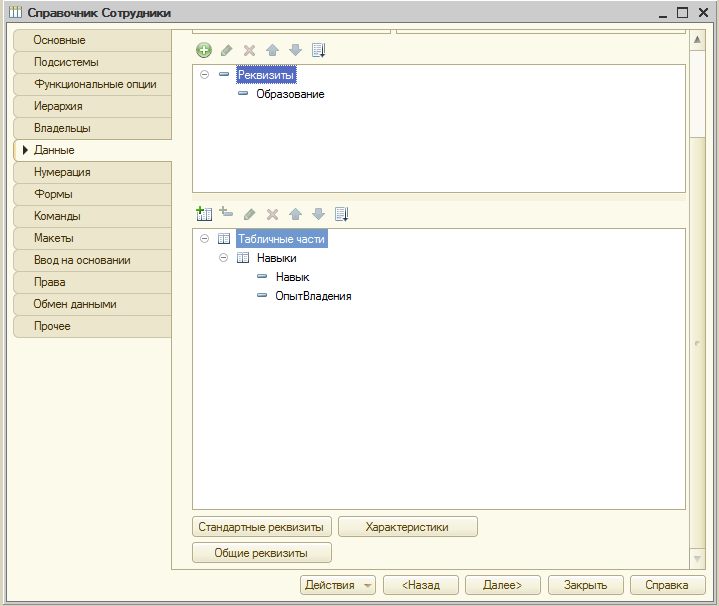
\includegraphics[width=110mm]{pic/employees}
  \caption{Структура справочника <<Сотрудники>>}
  \label{fig:employees}
\end{figure}

\begin{figure}[h!]
  \centering
  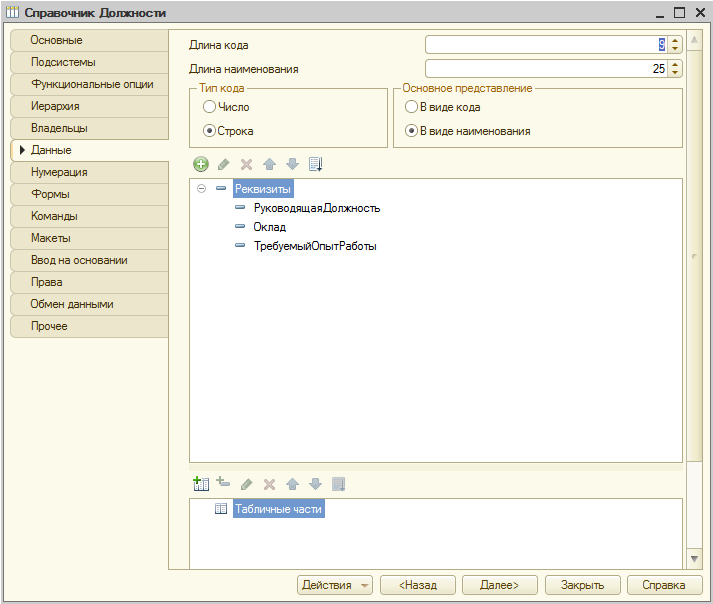
\includegraphics[width=110mm]{pic/positions}
  \caption{Структура справочника <<Должности>>}
  \label{fig:positions}
\end{figure}

\newpage

Справочник <<Навыки>> содержит стандартные реквезиты <<Код>> и
<<Наименование>>. Реквизиту <<Наименование>> установлен синоним <<Навык>>. 


\subsection{Создание документа}

Создание документов производится с помощью раздела <<Документы>>
панели <<Конфигурация>> режима <<Конфигуратор>>.
Для создания документа необходимо, щелкнув правой кнопкой мыши по этому
разделу, выбрать пункт <<Добавить>>. Далее в появившемся окне
следует определить имя и синоним документа.
После этого в разделе <<Данные>> необходимо определить структуру
хранимых данных путем добавления и указания свойств реквизитов
и табличных частей.

В разрабатываемой информационной системе документы используются для
регистрации фактов принятия сотрудников на определенную должность.

Структура документа <<ПриёмНаДолжность>>:
\begin{itemize}
  \item реквизит <<Должность>> (тип: СправочникСсылка.Должности);
  \item реквизит <<Оклад>> (тип: число, длина: 10);
  \item реквизит <<КоличествоСотрудников>> (тип: число, длина: 10);
  \item реквизит <<ОбщаяЗарплата>> (тип: число, длина: 10);
  \item табличная часть <<ПереченьСотрудников>>, содержащая поля
    <<Сотрудник>> (тип: СправочникСсылка.Сотрудники),
    <<Премия>> (тип: число, длина: 10),
    <<Образование>> (тип: ПеречисленияСсылка.Образования),
    <<Зарплата>> (тип: число, длина: 10).
\end{itemize}

Некоторые операции, производимые при заполнении нового документа,
можно оптимизировать. Например:
\begin{itemize}
  \item заполнение поля <<Оклад>> при выборе определенной должности;
  \item пересчёт полей <<КоличествоСотрудников>> и <<ОбщаяЗарплата>>
    при изменении табличной части; 
  \item пересчёт зарплаты для каждой строки табличной части <<ПереченьСотрудников>>.
\end{itemize}

\pagebreak

На рисунке~\ref{fig:form} приведен конструктор формы для
документа <<ПриёмНаДолжность>> в интерфейсе конфигуратора
СКД 1C:Предприятие.

\begin{figure}[h!]
  \centering
  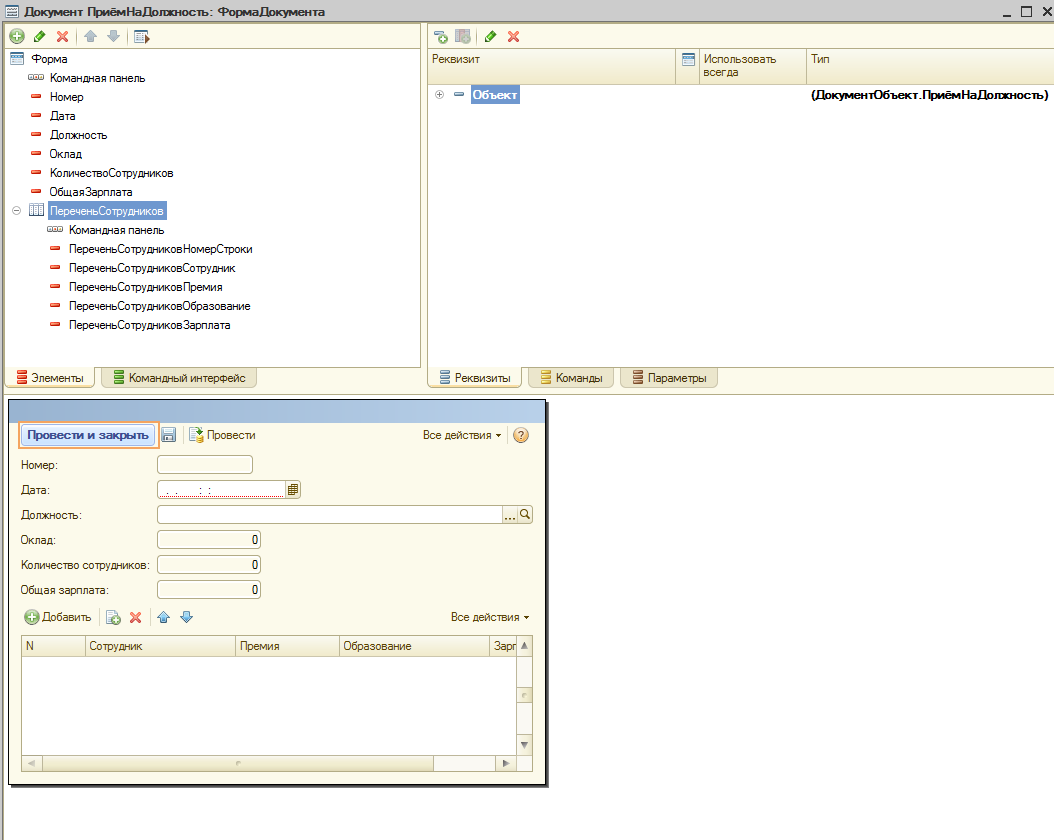
\includegraphics[width=150mm]{pic/form}
  \caption{Конструктор формы для документа <<ПриёмНаДолжность>>}
  \label{fig:form}
\end{figure}

Для автоматизации операций заполнения некоторых полей на форме документа
создадим обработчики событий <<ПриИзменении>> для следующих элементов формы:
\begin{itemize}
  \item Должность;
  \item ПереченьСотрудников;
  \item ПереченьСотрудниковСотрудник;
  \item ПереченьСотрудниковПремия.
\end{itemize}

\pagebreak

Обработчики приведенных событий <<ПриИзменении>> для указанных элементов,
а также вспомогательная процедура \texttt{ОбновитьСуммарныеДанные()}
приведены на рисунке~\ref{fig:form_event_handlers}.

\begin{figure}[h!]
  \centering
  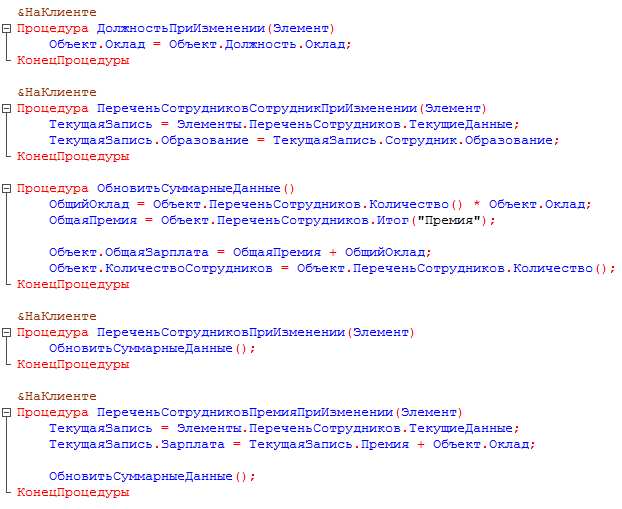
\includegraphics[width=150mm]{pic/form_event_handlers}
  \caption{Обработчики событий формы ввода данных \\
    документа <<ПриёмНаДолжность>>}
  \label{fig:form_event_handlers}
\end{figure}


\subsection{Создание регистра накопления}

Создание регистров накопления производится с помощью раздела
<<Регистры накопления>> панели <<Конфигурация>> режима <<Конфигуратор>>.
Для создания регистра накопления необходимо,
щелкнув правой кнопкой мыши по этому
разделу, выбрать пункт <<Добавить>>. Далее в появившемся окне
следует определить имя и синоним регистра.
После этого в разделе <<Данные>> необходимо определить структуру
хранимых данных путем добавления и указания свойств измерений и ресурсов.

\pagebreak

Для регистрации изменения зарплаты, премии и оклада сотрудников
создадим регистр накопления <<КоличествоСотрудников>> с измерениями
<<Должность>> (тип: СправочникСсылка.Должности),
<<Сотрудник>> (тип: СправочникСсылка.Сотрудники)
и ресурсами
<<Оклад>> (тип: число, длина: 10),
<<Премия>> (тип: число, длина: 10),
<<Зарплата>> (тип: число, длина: 10),
как показано на рисунке~\ref{fig:register}.

\begin{figure}[h!]
  \centering
  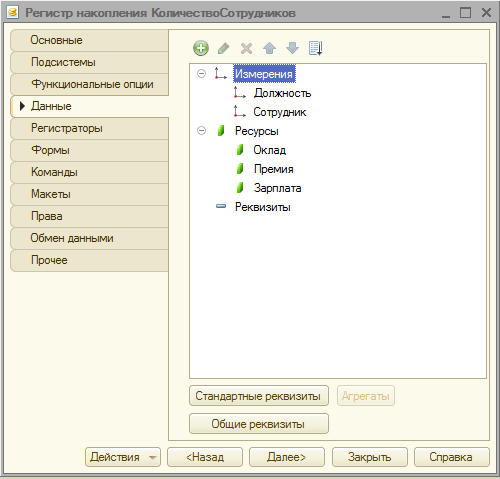
\includegraphics[width=120mm]{pic/register}
  \caption{Структура регистра накопления \\ <<КоличествоСотрудников>>}
  \label{fig:register}
\end{figure}

Для данного регистра в качестве документа-регистратора
установим документ <<ПриёмНаДолжность>>.
Это можно сделать с помощью конструктора движения регистров,
расположенного на вкладке <<Движения>> свойств документа

\pagebreak

На рисунках~\ref{fig:register_registers}~и~\ref{fig:register_document_drive} продемонстрирован
процесс настройки регистра накопления <<КоличествоСотрудников>>.

\begin{figure}[h!]
  \centering
  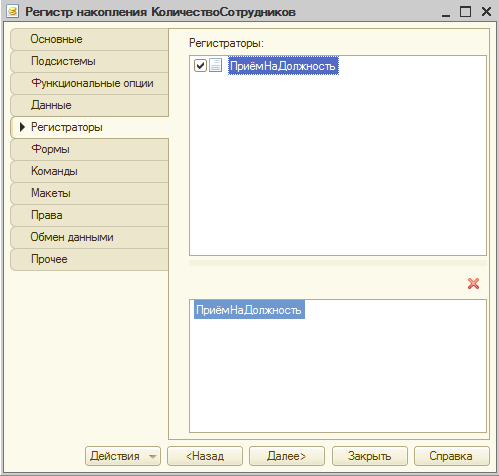
\includegraphics[width=100mm]{pic/register_registers}
  \caption{Установление регистратора (документа) для регистра <<ПоступлениеТоваров>>}
  \label{fig:register_registers}
\end{figure}

\begin{figure}[h!]
  \centering
  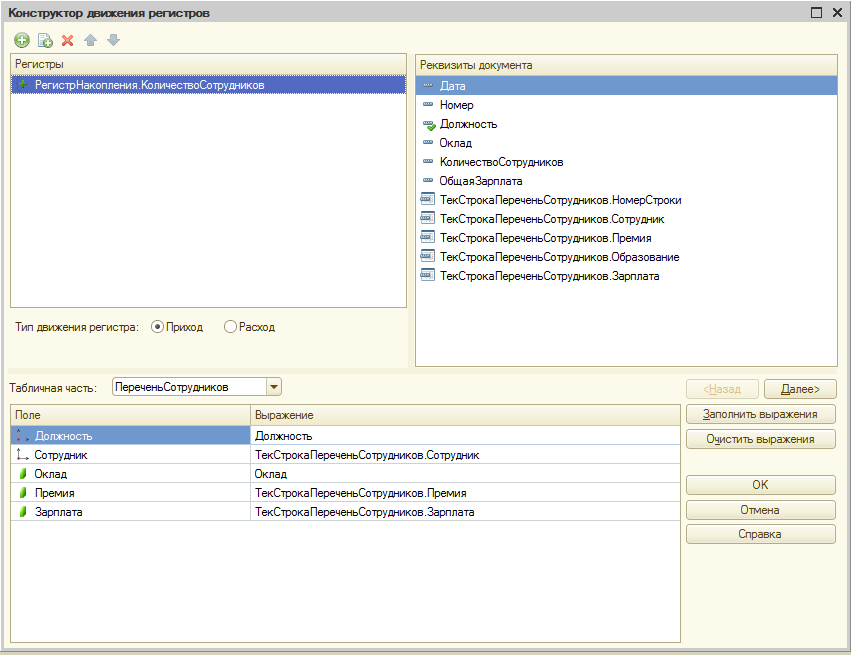
\includegraphics[width=100mm]{pic/register_document_drive}
  \caption{Параметры регистрации движения документа <<ПриёмНаДолжность>>}
  \label{fig:register_document_drive}
\end{figure}

\pagebreak


\subsection{Создание отчетов}

Создание отчетов производится с помощью раздела
<<Отчеты>> панели <<Конфигурация>> режима <<Конфигуратор>>.
Для создания отчета необходимо,
щелкнув правой кнопкой мыши по этому
разделу, выбрать пункт <<Добавить>>. Далее в появившемся окне
следует определить имя и синоним отчета.

Для настройки набора и способа отображения данных в
автоматическом режиме будем использовать
мастер редактирования схемы компоновки данных,
запуск которого производится нажатием кнопки
<<Открыть схему компоновки данных>>, расположенной
на вкладке <<Основные>> окна свойств отчета.

Для выбора данных, отображаемых в отчете, будем использовать
конструктор запроса, запуск которого производится нажатием кнопки
<<Конструктор запроса...>>, расположенной
на вкладке <<Наборы данных>> окна
мастера редактирования схемы компоновки данных отчета.

Для настройки способа отображения данных в отчете будем использовать
конструктор настроек отчета, запуск которого производится нажатием кнопки
<<Конструктор настроек>>, расположенной
на вкладке <<Настройки>> окна
мастера редактирования схемы компоновки данных отчета.

Создадим отчет о приёме сотрудников на работу,
содержащий данные о должностях, сотрудниках и зарплате,
сгруппированные по должности.
Для этого в режиме конфигуратора СКД 1С:Предприятие создадим отчет
<<ОтчетПоНаймуСотрудников>>, с помощью конструктора запросов
определим набор данных, извлекаемых из информационной системы:
\begin{itemize}
  \item <<КоличествоСотрудниковОстатки.Должность>>,
  \item <<КоличествоСотрудниковОстатки.ЗарплатаОстаток>>,
  \item <<КоличествоСотрудниковОстатки.Сотрудник>>.
\end{itemize}

\pagebreak

Пример создания отчёта с использованием конструктора приведен
на рисунках~\ref{fig:report_constructor}~и~\ref{fig:report_scheme}.

\begin{figure}[h!]
  \centering
  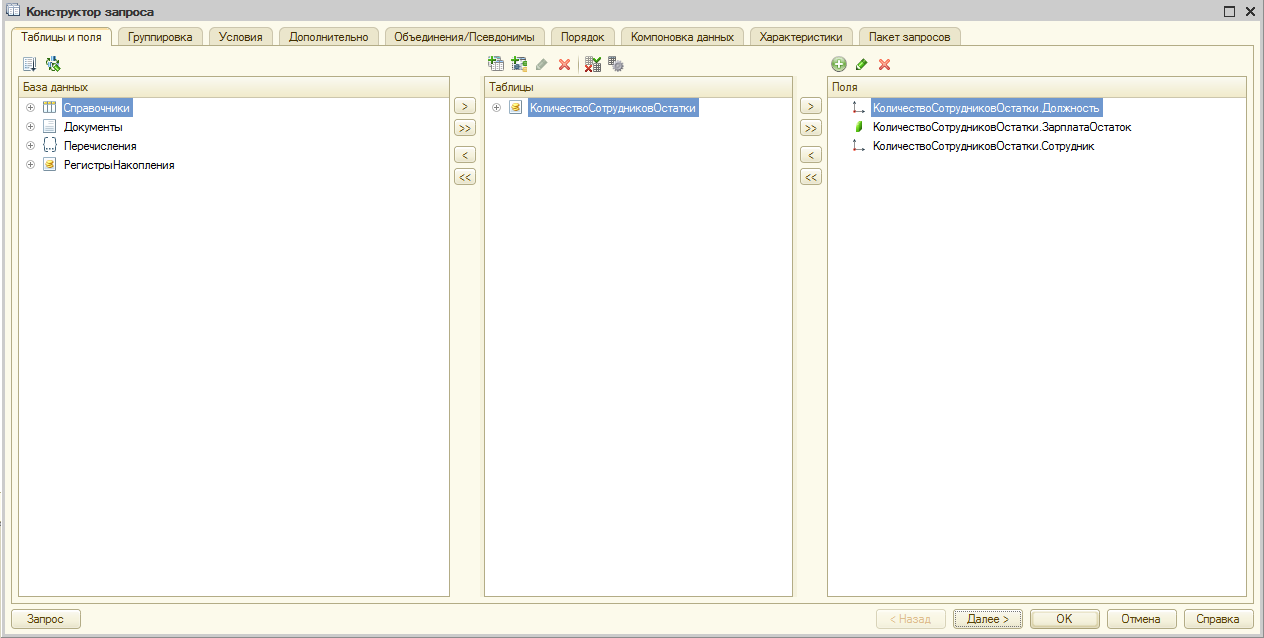
\includegraphics[width=160mm]{pic/report_constructor}
  \caption{Конструктор запросов отчета \\ <<ОтчетПоНаймуСотрудников>>}
  \label{fig:report_constructor}
\end{figure}

\begin{figure}[h!]
  \centering
  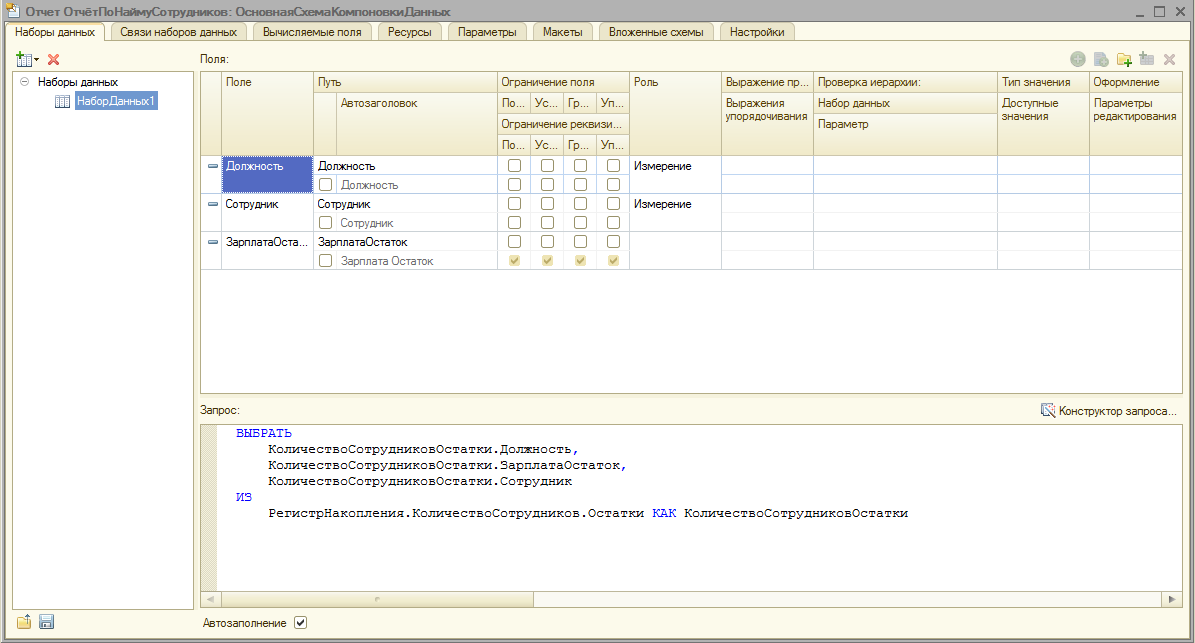
\includegraphics[width=160mm]{pic/report_scheme}
  \caption{Схема компоновки данных отчета \\ <<ОтчетПоНаймуСотрудников>>}
  \label{fig:report_scheme}
\end{figure}

\pagebreak

Пример разработанного отчета приведен на рисунке~\ref{fig:report_results}.
\begin{figure}[h!]
  \centering
  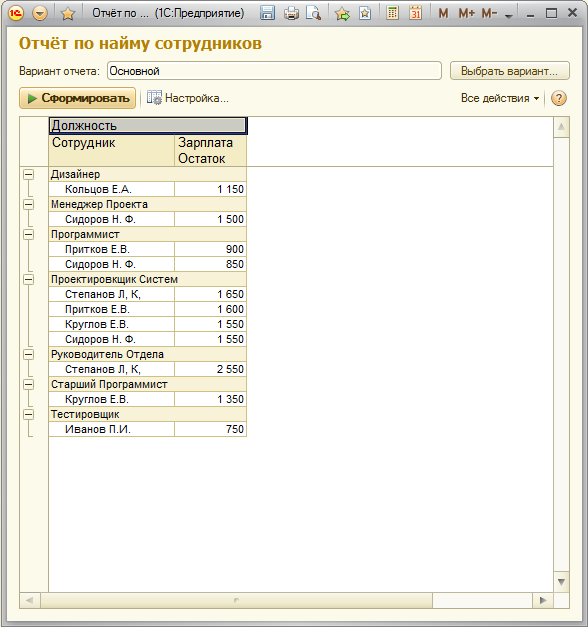
\includegraphics[width=130mm]{pic/report_results}
  \caption{Отчет <<ОтчетПоНаймуСотрудников>>}
  \label{fig:report_results}
\end{figure}

Создадим отчёт в виде диаграммы, отражающий величину заработной платы
по должностям. Для этого в режиме конфигуратора СКД 1С:Предприятие
создадим отчет <<ОтчетДиаграмма>>, с помощью конструктора запросов
определим набор данных, извлекаемых из информационной системы.

\pagebreak

На рисунке~\ref{fig:diagram_scheme} приведена схема компоновки данных отчета.
\begin{figure}[h!]
  \centering
  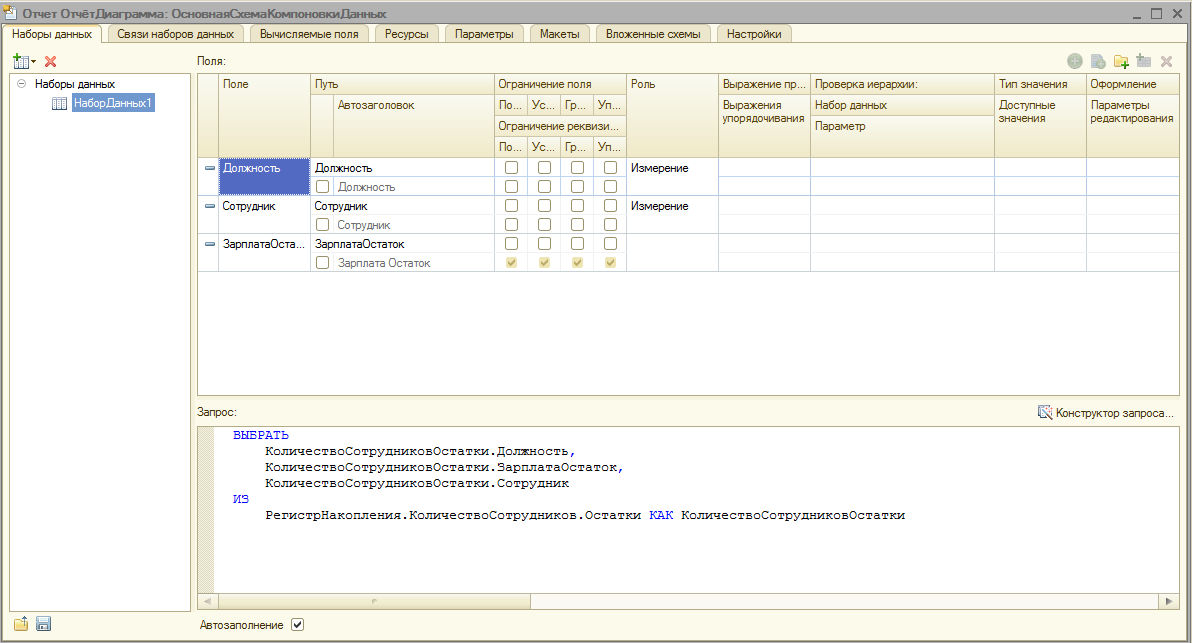
\includegraphics[width=110mm]{pic/diagram_scheme}
  \caption{Конструктор запросов отчета \\ <<ОтчетДиаграмма>>}
  \label{fig:diagram_scheme}
\end{figure}

Далее перейдем на вкладку <<Настройки>>, c помощью конструктора
настроек компоновки данных определим поля, отображаемые на диаграмме,
как показано на рисунке~\ref{fig:diagramm_constructor}.
\begin{figure}[h!]
  \centering
  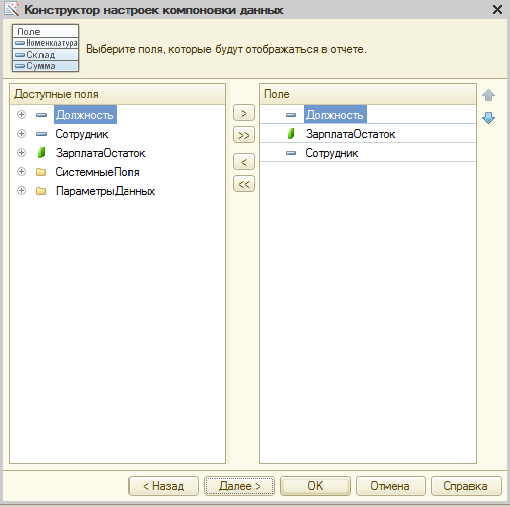
\includegraphics[width=90mm]{pic/diagramm_constructor}
  \caption{Конструктор настроек компоновки данных диаграммы <<ОтчетДиаграмма>>}
  \label{fig:diagramm_constructor}
\end{figure}

\pagebreak

Пример разработанного отчета приведен на рисунке~\ref{fig:diagram_results}.

\begin{figure}[h!]
  \centering
  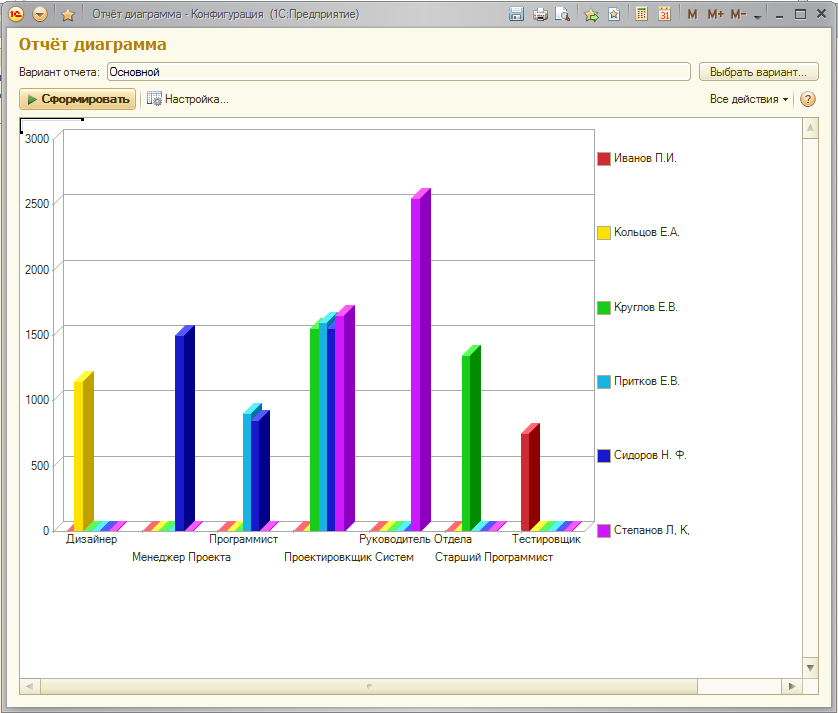
\includegraphics[width=140mm]{pic/diagram_results}
  \caption{Диаграмма <<ОтчетДиаграмма>>}
  \label{fig:diagram_results}
\end{figure}

Отчёт демонстрирует размер зарплаты сотрудников в зависимости от занимаемой
должности. Стоит отметить, что в рамках разрабатываемой системы считается,
что один сотрудник может занимать несколько должностей.

\pagebreak

\subsection{Создание запросов}

Для демонстрации работы запросов в СКД 1С:Предприятие будем
использовать обработки.
Создание обработки производится с помощью раздела
<<Обработки>> панели <<Конфигурация>> режима <<Конфигуратор>>.
Для создания обработки необходимо,
щелкнув правой кнопкой мыши по этому
разделу, выбрать пункт <<Добавить>>. Далее в появившемся окне
следует определить имя и синоним обработки;
на вкладке <<Формы>> создать и настроить форму обработки,
установив требуемые элементы управления, затем на вкладке
<<Модуль>> ввести программный код.


% СотрудникиПоНавыку

Создадим запрос, отображающий перечень сотрудников, имеющих определенный навык.
В качестве параметра запроса будет выступать <<Навык>>.

Для этого создадим обработку <<СотрудникиПоНавыку>>
с дополнительным реквизитом <<ВводНавыка>> и командой
<<ВыбратьДанные>>, как показано на рисунке~\ref{fig:employees_by_skill_query}.
На вкладке <<Модуль>> формы назначим обработчик нажатия кнопки
<<ВыбратьДанные>>.

Для реквизита <<ВводНавыка>> установим тип данных --- СправочникСсылка.Навыки,
с помощью мыши перенесём реквизит на форму, таким образом позволим осуществлять
выбор навыка пользователем.

\begin{figure}[h!]
  \centering
  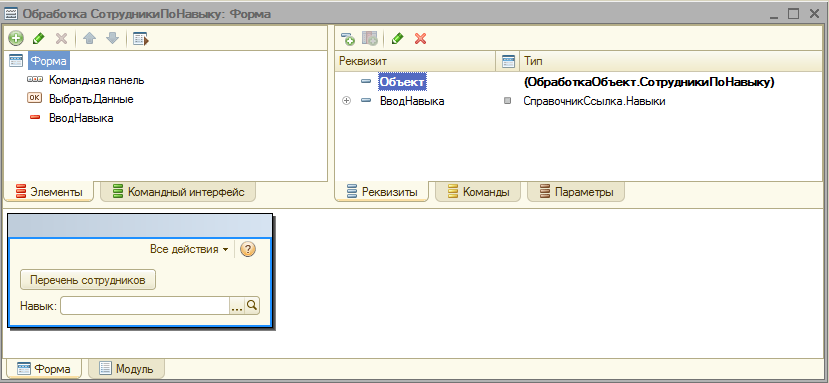
\includegraphics[width=150mm]{pic/employees_by_skill_query}
  \caption{Форма обработки <<СотрудникиПоНавыку>>}
  \label{fig:employees_by_skill_query}
\end{figure}

\pagebreak

На рисунках~\ref{fig:employees_by_skill_code}~и~\ref{fig:employees_by_skill_results}
изображены модуль формы обработки <<СотрудникиПоНавыку>> и результаты её выполнения.
\begin{figure}[h!]
  \centering
  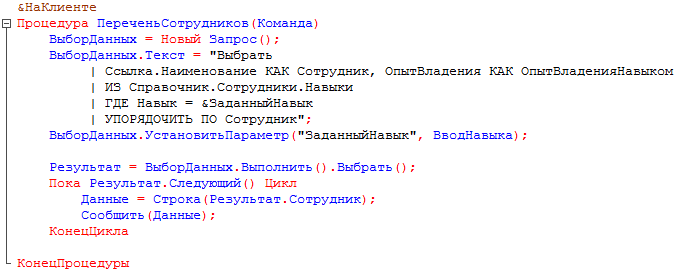
\includegraphics[width=160mm]{pic/employees_by_skill_code}
  \caption{Модуль формы обработки <<СотрудникиПоНавыку>>}
  \label{fig:employees_by_skill_code}
\end{figure}

\begin{figure}[h!]
  \centering
  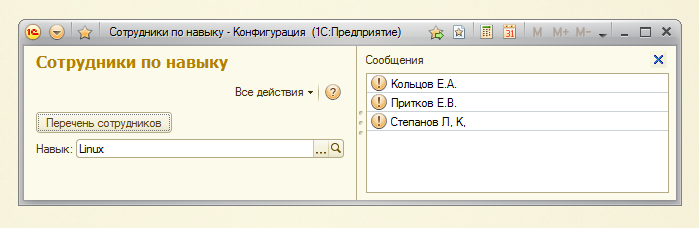
\includegraphics[width=160mm]{pic/employees_by_skill_results}
  \caption{Результат выполнения обработки <<СотрудникиПоНавыку>>}
  \label{fig:employees_by_skill_results}
\end{figure}


% Сотрудники с максимальной Зарплатой

Создадим запрос, отображающий перечень (первые три из списка) сотрудников
с максимальной зарплатой с указанием ФИО сотрудника,
должности и зарплаты.
Для этого создадим обработку <<СотрудникиСВысокойЗарплатой>>
с командой <<ВыбратьДанные>>.

\pagebreak

На рисунках~\ref{fig:first_three_form}--\ref{fig:first_three_results} приведены
форма обработки <<СотрудникиСВысокойЗарплатой>>, её модуль и
результаты выполнения обработки.

\begin{figure}[h!]
  \centering
  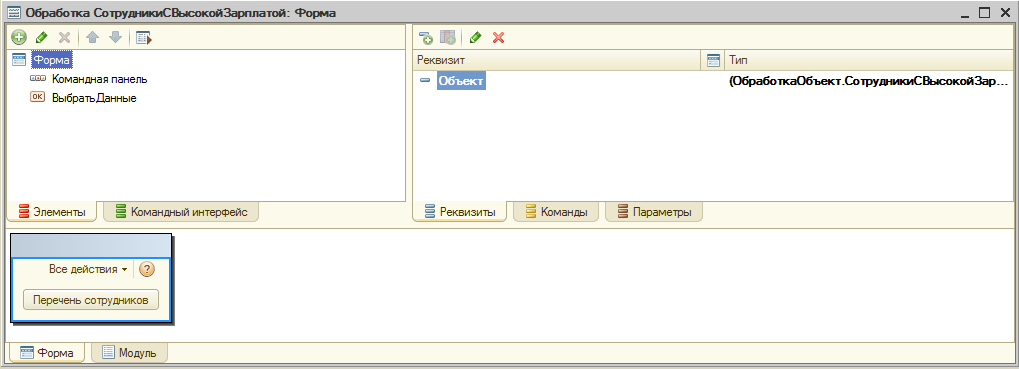
\includegraphics[width=160mm]{pic/first_three_form}
  \caption{Форма обработки <<СотрудникиСВысокойЗарплатой>>}
  \label{fig:first_three_form}
\end{figure}

\begin{figure}[h!]
  \centering
  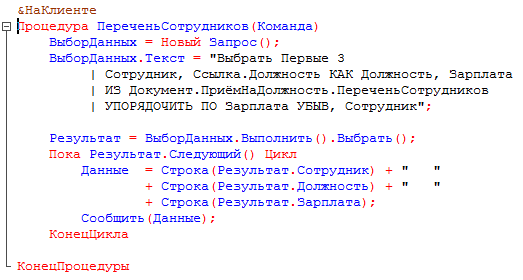
\includegraphics[width=100mm]{pic/first_three_code}
  \caption{Модуль формы обработки \\ <<СотрудникиСВысокойЗарплатой>>}
  \label{fig:first_three_code}
\end{figure}

\begin{figure}[h!]
  \centering
  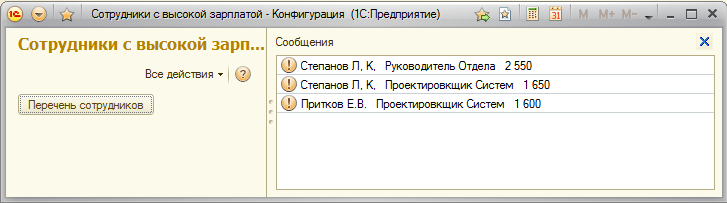
\includegraphics[width=140mm]{pic/first_three_results}
  \caption{Результат выполнения обработки \\ <<СотрудникиСВысокойЗарплатой>>}
  \label{fig:first_three_results}
\end{figure}

\pagebreak


% ДолжностиВышеЗаданнойЗарплаты 

Создадим обработку, отображающую перечень сотрудников и должностей, имеющих зарплату
выше некоторой минимальной величины, которую задаёт пользователь.

Для этого создадим обработку <<ДолжностиВышеЗаданнойЗарплаты>>
с дополнительным реквизитом <<ВводЗарплаты>> и командой
<<ПереченьДолжностей>>, как показано на рисунке~\ref{fig:by_min_salary_form}.
На вкладке <<Модуль>> формы назначим обработчик нажатия кнопки
<<ПереченьДолжностей>>, приведенный на рисунке~\ref{fig:by_min_salary_code}.

Для реквизита <<ВводЗарплаты>> установим тип данных --- число,
синоним --- <<Минимальная Зарплата>>, с помощью мыши
перенесём реквизит на форму, таким образом позволим осуществлять
ввод некоторого числа (минимальной зарплаты) пользователем.

\begin{figure}[h!]
  \centering
  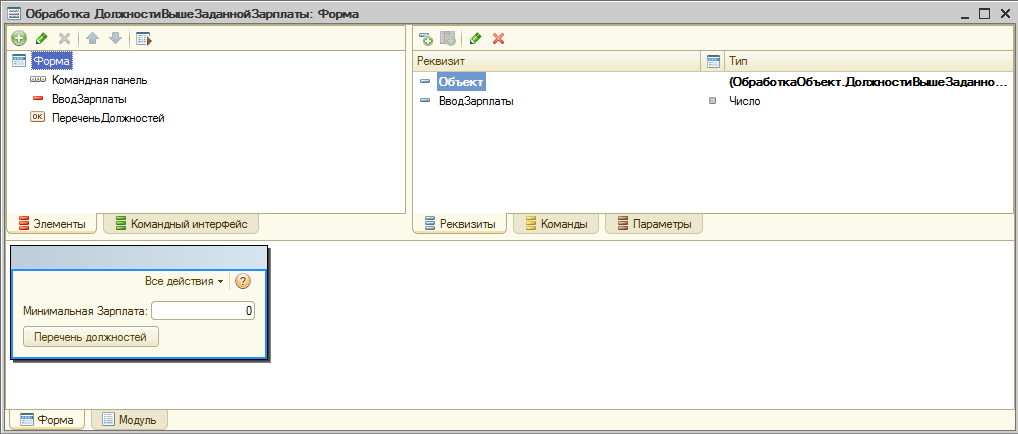
\includegraphics[width=140mm]{pic/by_min_salary_form}
  \caption{Форма обработки <<ДолжностиВышеЗаданнойЗарплаты>>}
  \label{fig:by_min_salary_form}
\end{figure}

\begin{figure}[h!]
  \centering
  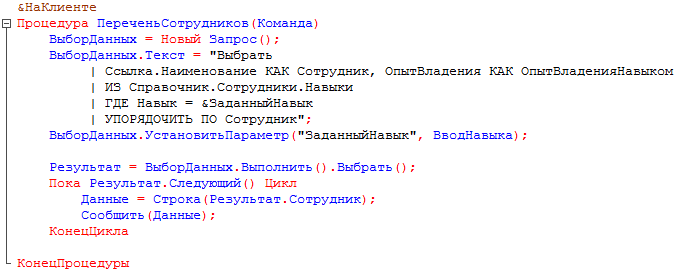
\includegraphics[width=140mm]{pic/employees_by_skill_code}
  \caption{Модуль формы обработки <<ДолжностиВышеЗаданнойЗарплаты>>}
  \label{fig:by_min_salary_code}
\end{figure}

На рисунке~\ref{fig:by_min_salary_results} изображен и результат выполнения
обработки <<ДолжностиВышеЗаданнойЗарплаты>>.
\begin{figure}[h!]
  \centering
  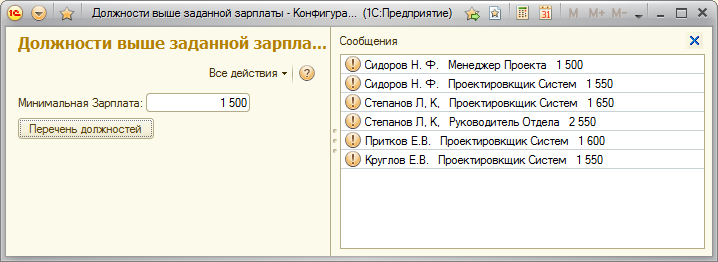
\includegraphics[width=160mm]{pic/by_min_salary_results}
  \caption{Результат выполнения обработки <<ДолжностиВышеЗаданнойЗарплаты>>}
  \label{fig:by_min_salary_results}
\end{figure}


% ЗарплатаПоДолжностям (СУММА, КОЛИЧЕСТВО)

Создадим запрос, отображающий суммарную зарплату по каждой должности
с указанием количества занятых на этой должности сотрудников.

Для этого создадим обработку <<ЗарплатаПоДолжностям>>
с командой <<ВыбратьДанные>>,
как показано на рисунке~\ref{fig:salary_by_positions_form}.
\begin{figure}[h!]
  \centering
  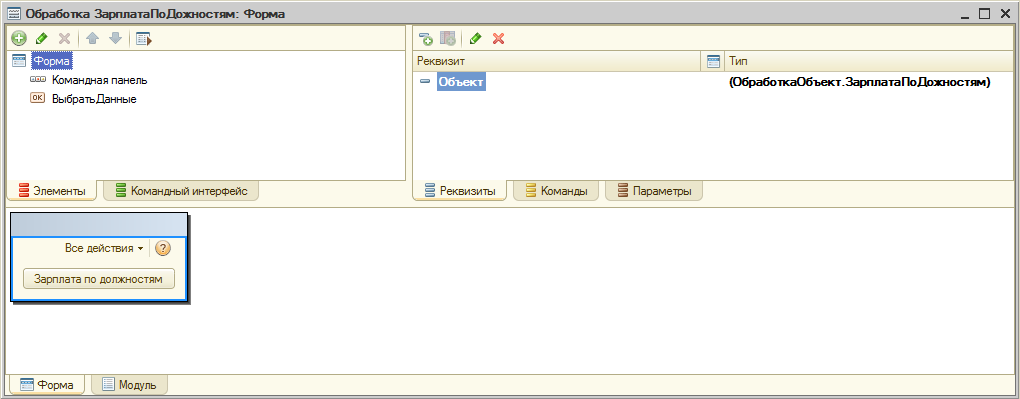
\includegraphics[width=160mm]{pic/salary_by_positions_form}
  \caption{Форма обработки <<ЗарплатаПоДолжностям>>}
  \label{fig:salary_by_positions_form}
\end{figure}

\pagebreak

На вкладке <<Модуль>> формы назначим обработчик нажатия кнопки
<<ВыбратьДанные>>, как показано на рисунке~\ref{fig:salary_by_positions_code}.
На рисунке~\ref{fig:salary_by_positions_results} приведен результат
выполнения обработки.
\begin{figure}[h!]
  \centering
  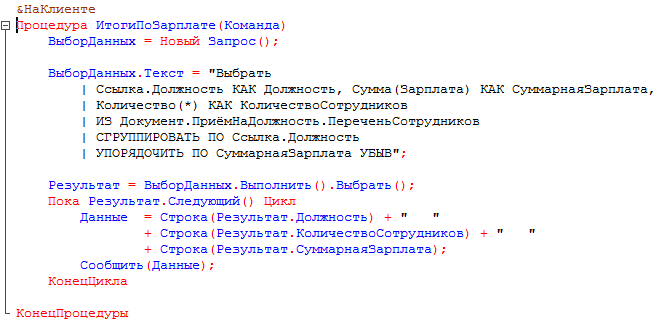
\includegraphics[width=150mm]{pic/salary_by_positions_code}
  \caption{Модуль формы обработки \\ <<ЗарплатаПоДолжностям>>}
  \label{fig:salary_by_positions_code}
\end{figure}

\begin{figure}[h!]
  \centering
  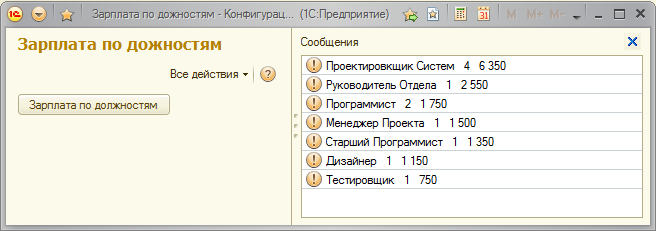
\includegraphics[width=150mm]{pic/salary_by_positions_results}
  \caption{Результат выполнения обработки \\ <<ЗарплатаПоДолжностям>>}
  \label{fig:salary_by_positions_results}
\end{figure}


% ЗарплатаИтоги

Создадим запрос, отображающий информацию о работниках,
их должностях, оклада, премии и зарплаты сотрудников.
Необходимо предусмотреть вычисление итогов по категории
<<Должность>>.

\pagebreak

Для решения этой задачи создадим обработку <<ЗарплатаИтоги>>
с командой <<ВыбратьДанные>>,
как показано на рисунке~\ref{fig:salary_amount_form}.

На вкладке <<Модуль>> формы назначим обработчик нажатия кнопки
<<ВыбратьДанные>>, как показано на рисунке~\ref{fig:salary_amount_code}.

\begin{figure}[h!]
  \centering
  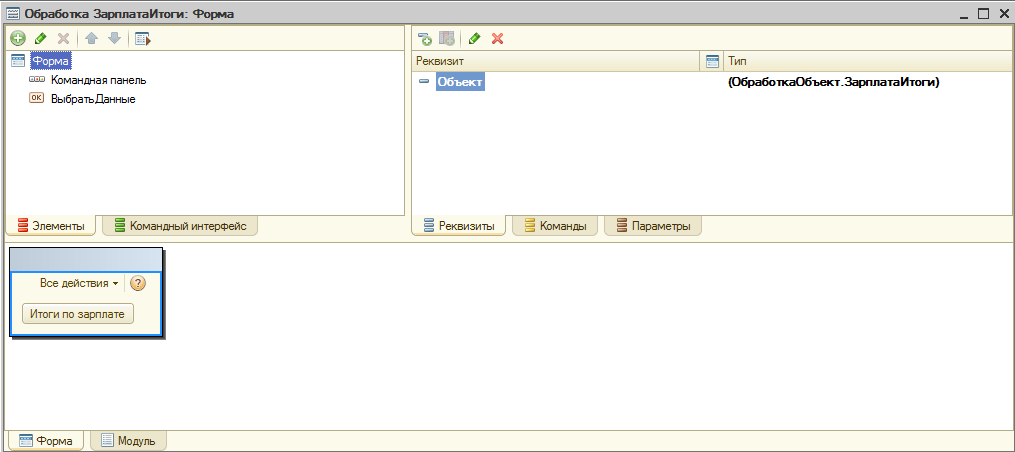
\includegraphics[width=150mm]{pic/salary_amount_form}
  \caption{Форма обработки <<ЗарплатаИтоги>>}
  \label{fig:salary_amount_form}
\end{figure}

\begin{figure}[h!]
  \centering
  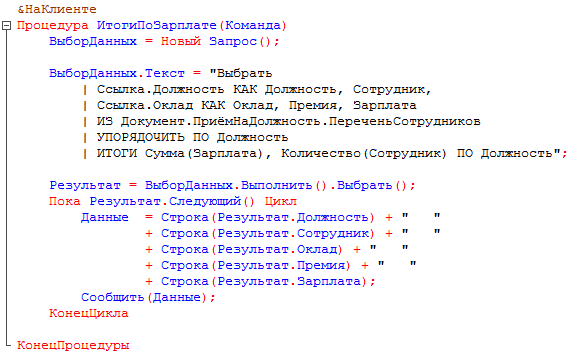
\includegraphics[width=160mm]{pic/salary_amount_code}
  \caption{Модуль формы обработки \\ <<ЗарплатаИтоги>>}
  \label{fig:salary_amount_code}
\end{figure}

\pagebreak

Результат работы обработки <<ЗарплатаИтоги>> приведен
на рисунке~\ref{fig:salary_amount_results}.
\begin{figure}[h!]
  \centering
  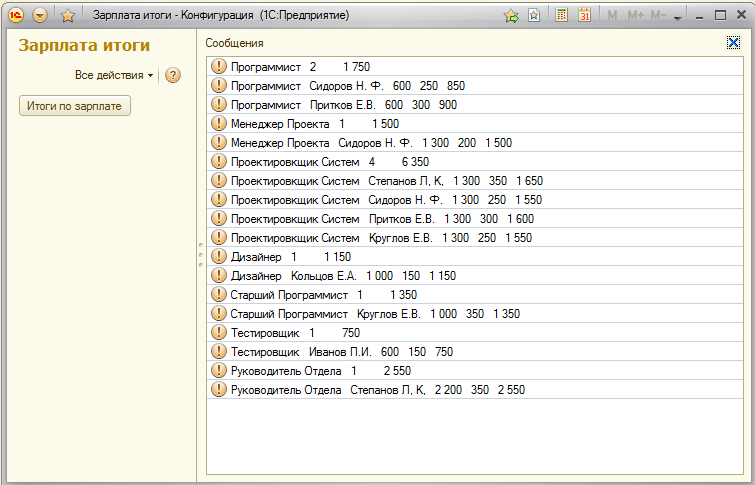
\includegraphics[width=160mm]{pic/salary_amount_results}
  \caption{Результат выполнения обработки <<ЗарплатаИтоги>>}
  \label{fig:salary_amount_results}
\end{figure}


% Руководители

Создадим запрос, отображающий перечень руководящих должностей
с указанием заработной платы. Для этого воспользуемся связыванием
Справочника и Документа по типу <<ЛЕВОЕ СОЕДИНЕНИЕ>>.
Для этого создадим обработку <<Руководители>>
с командой <<ВыбратьРуководителей>>, как показано на рисунке~\ref{fig:managers_form}
\begin{figure}[h!]
  \centering
  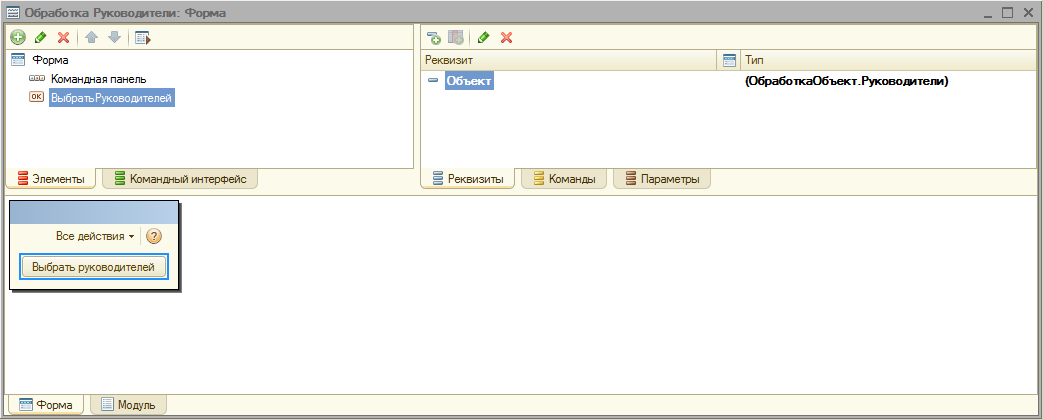
\includegraphics[width=130mm]{pic/managers_form}
  \caption{Форма обработки <<Руководители>>}
  \label{fig:managers_form}
\end{figure}

\pagebreak

На вкладке <<Модуль>> назначим обработчик нажатия кнопки <<ВыбратьРуководителей>>.
Обработчик нажатия кнопки <<ВыбратьРуководителей>> и результат выполения обработки
приведены на рисунках~\ref{fig:managers_code}~и~\ref{fig:managers_results}.
\begin{figure}[h!]
  \centering
  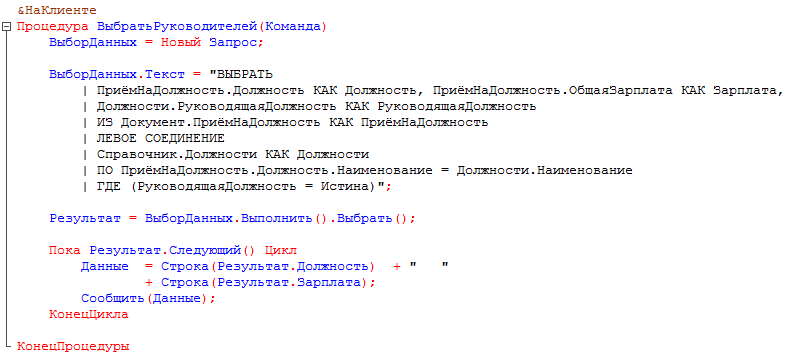
\includegraphics[width=150mm]{pic/managers_code}
  \caption{Модуль формы обработки <<Руководители>>}
  \label{fig:managers_code}
\end{figure}
\begin{figure}[h!]
  \centering
  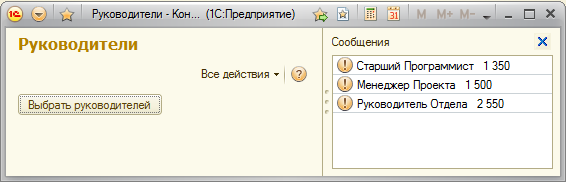
\includegraphics[width=140mm]{pic/managers_results}
  \caption{Результат выполнения обработки <<Руководители>>}
  \label{fig:managers_results}
\end{figure}

% Руководители

Создадим запрос, отображающий потоки денежных средств сгруппированных
по должностям с указанием оклада, премии и заработной платы.
Требуется предусмотреть представление данных в виде отчета.

\pagebreak

Для этого создадим обработку <<ДолжностиОтчет>>
с командой <<ВыбратьДанные>>, как показано на рисунке~\ref{fig:positions_report_form}
\begin{figure}[h!]
  \centering
  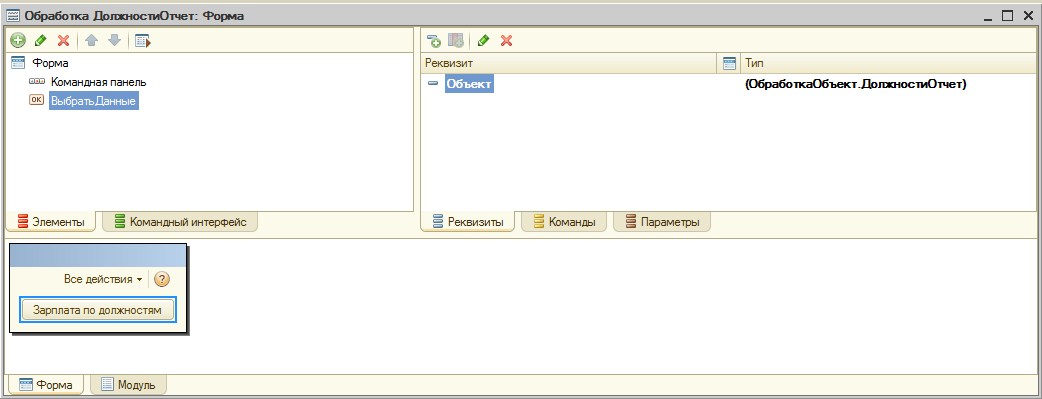
\includegraphics[width=140mm]{pic/positions_report_form}
  \caption{Форма обработки <<ДолжностиОтчет>>}
  \label{fig:positions_report_form}
\end{figure}

На вкладке <<Модуль>> назначим обработчик нажатия кнопки <<ВыбратьДанные>>.
Обработчик нажатия кнопки <<ВыбратьРуководителей>> представлен на
рисунке~\ref{fig:positions_report_code}.
\begin{figure}[h!]
  \centering
  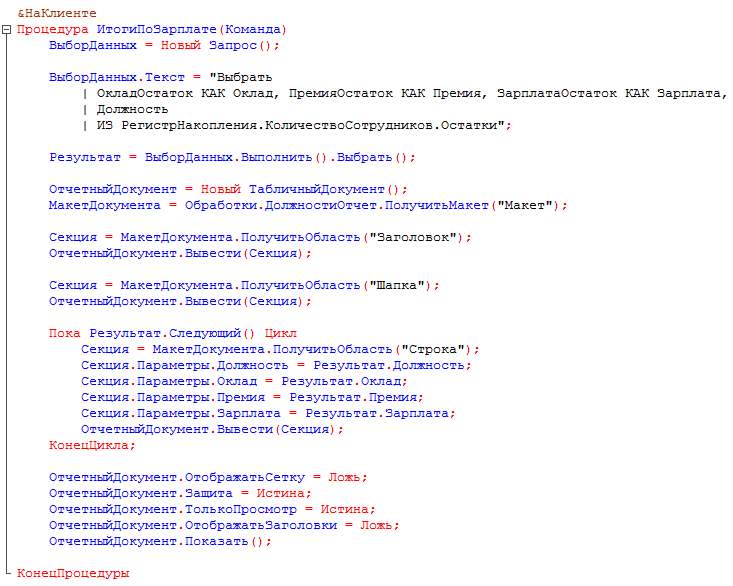
\includegraphics[width=140mm]{pic/positions_report_code}
  \caption{Модуль формы обработки <<ДолжностиОтчет>>}
  \label{fig:positions_report_code}
\end{figure}

\pagebreak

На рисунках~\ref{fig:positions_report_template}~и~\ref{fig:positions_report_results}
приведены подготовленный макет отчета и результат выполнения обработки <<ДолжностиОтчет>>.
\begin{figure}[h!]
  \centering
  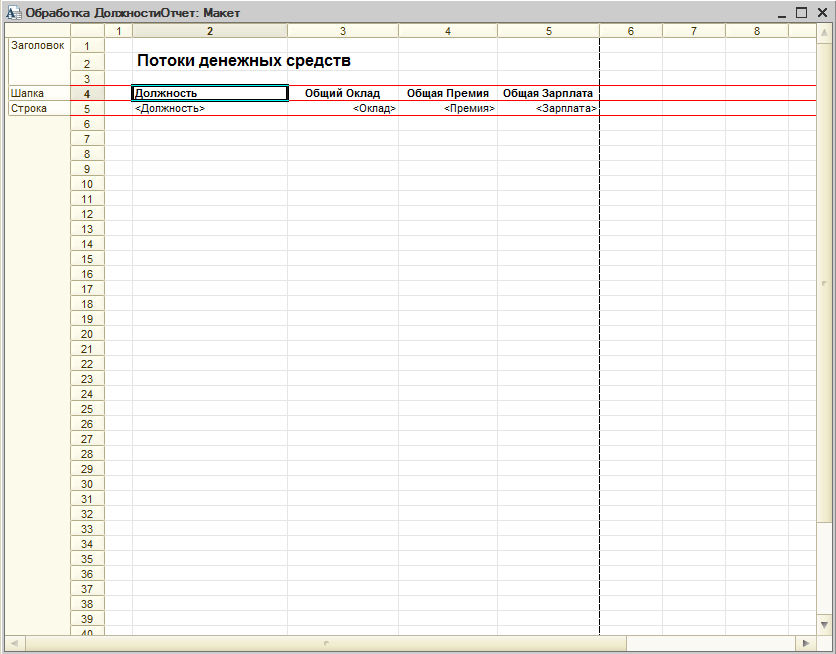
\includegraphics[width=110mm]{pic/positions_report_template}
  \caption{Макет отчёта обработки <<ДолжностиОтчет>>}
  \label{fig:positions_report_template}
\end{figure}
\begin{figure}[h!]
  \centering
  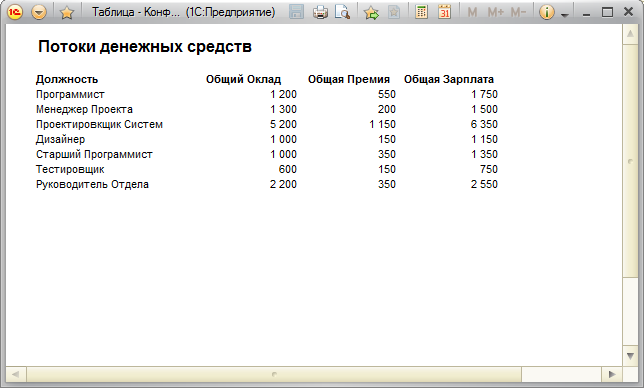
\includegraphics[width=140mm]{pic/positions_report_results}
  \caption{Макет отчёта обработки <<ДолжностиОтчет>>}
  \label{fig:positions_report_results}
\end{figure}
